\documentclass{standalone}
\usepackage{tikz}
\usepackage{kpfonts}

\usetikzlibrary{decorations.pathreplacing}

\begin{document}
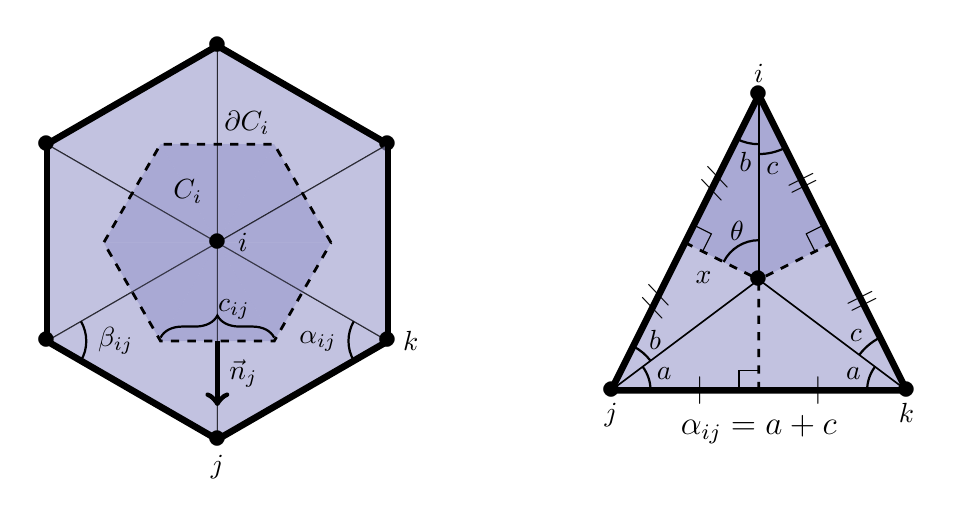
\begin{tikzpicture}[scale=1.25]
	\definecolor{facecol}{rgb}{0.6,0.6,0.8}
	\coordinate (i) at (0, 0);
	\foreach \a in {30, 90, ..., 330} {
		\coordinate (j) at ({\a-30}:{2/sqrt(3)});
		\coordinate (k) at ({\a+30}:{2/sqrt(3)});
		\fill[facecol, opacity=.6, ] (i) -- (j) -- (k) -- cycle;
		
		\coordinate (j) at ({\a}:2);
		\coordinate (k) at ({\a+60}:2);
		\draw[fill=facecol, opacity=.6] (i) -- (j) -- (k) -- cycle;
		\draw[line width=2.4pt] (j) -- (k);
		\node at (j) {\Large $\bullet$};
	}
	\node at (i) {\Large $\bullet$};
	\draw[line width=1pt, dashed] (0:{2/sqrt(3)}) \foreach \a in {60, 120, ..., 360} {
		-- ({\a}:{2/sqrt(3)})
	};
	\node[right=4pt] at (i) {$i$};
	\node[below=2pt] at (0, -2) {$j$};
	\node[right=2pt] at ({2*cos(30)}, {-2*sin(30)}) {$k$};
	\node[] at (120:.6) {$C_i$};
	\node[above] at (0.3, 1) {$\partial C_i$};
	\draw[thick] (-150:2){}+(-30:0.4) arc (-30:30:0.4);
	\node[right=15pt] at (210:2) {$\beta_{ij}$};
	\draw[thick] (-30:2){}+(-150:0.4) arc (-150:-210:0.4);
	\node[left=15pt] at (-30:2) {$\alpha_{ij}$};
	\draw[line width=2pt, ->] (0, -1) -- node[right] {$\vec{n}_j$} (0, -1.66);
	\draw[decorate, decoration={brace,amplitude=8pt}, thick, yshift=1pt] (-120:{2/sqrt(3)}) -- node[above=3pt] {$\hspace{12pt} c_{ij}$} (-60:{2/sqrt(3)});
	
	\coordinate (i) at (4, -1.5);
	\coordinate (j) at (7, -1.5);
	\coordinate (k) at (5.5, 1.5);
	\coordinate (c) at (5.5, -.375);
	\coordinate (midi) at (4.75, 0);
	\coordinate (midk) at (6.25, 0);
	\fill[fill=facecol, opacity=.6] (i) -- (j) -- (k) -- cycle;
	\fill[fill=facecol, opacity=.6] (k) -- (midi) -- (c) -- (midk) -- cycle;
	\draw[line width=2.4pt] (i) -- node[pos=.3] {$|$} node[pos=.7] {$|$} (j) -- node[pos=.3, sloped] {$||$} node[pos=.7, sloped] {$||$} (k) -- node[pos=.3, sloped] {$//$} node[pos=.7, sloped] {$//$} (i);
	\draw[line width=1pt, dashed] (5.5, -1.5) -- (c);
	\draw[] (5.3, -1.5) -- (5.3, -1.3) -- (5.5, -1.3);
	\draw[line width=1pt, dashed] (midi) -- node[below left] {$x$} (c);
	\draw[] (midi){}++({atan(2)}:.2) --++ ({atan(2)-90}:.2) --++ ({180+atan(2)}:.2);
	\draw[line width=1pt, dashed] (midk) -- (c);
	\draw[] (midk){}++({180-atan(2)}:.2) --++ ({-90-atan(2)}:.2) --++ ({-atan(2)}:.2);
	\draw[line width=.6pt] (i) -- (c);
	\draw[line width=.6pt] (j) -- (c);
	\draw[line width=.6pt] (k) -- (c);
	\draw (i) node {\Large $\bullet$} (j) node {\Large $\bullet$} (k) node {\Large $\bullet$} (c) node {\Large $\bullet$};
	\draw (i) node[below=1pt] {$j$} (j) node[below=1pt] {$k$} (k) node[above=1pt] {$i$};
	\node at (5.5, -1.9) {\large $\alpha_{ij}=a+c$};
	\draw[thick] (i){}+(0.4,0) arc (0:{atan(3/4)}:0.4) node[right, pos=.7] {$a$};
	\draw[thick] (i){}+({atan(3/4)}:0.5) arc ({atan(3/4)}:{atan(2)}:0.5) node[above right=-2pt, pos=.4] {$b$};
	\draw[thick] (j){}+(-0.4,0) arc (180:{180-atan(3/4)}:0.4) node[left, pos=.7] {$a$};
	\draw[thick] (j){}+({180-atan(3/4)}:0.6) arc ({180-atan(3/4)}:{180-atan(2)}:0.6) node[above left=-2pt, pos=.4] {$c$};
	\draw[thick] (k){}+(0,-0.5) arc (-90:{-90-atan(.5)}:0.5) node[below, pos=.6] {$b$};
	\draw[thick] (k){}+(0,-0.6) arc (-90:{-90+atan(.5)}:0.6) node[below, pos=.5] {$c$};
	\draw[thick] (c){}+({180-atan(.5)}:.4) arc ({180-atan(.5)}:90:0.4) node[above left=-3pt, pos=.7] {$\theta$};
\end{tikzpicture}
\end{document}